\chapter{Implementation}

This chapter extends the design presented in Chapter \ref{chap:design}, focusing on implementing the Proof Key for Code Exchange (PKCE) authorisation flow for a dual-tenant environment. Using the multi-database architecture proposed in the design (refer to Figure \ref{fig:deployment_diagram_dual}), this implementation builds a foundational prototype of the OAuth 2.0 Authorisation Code flow with PKCE, adapted for a multi-tenant, serverless infrastructure. By leveraging modern, cloud-native technologies—including Node.js, TypeScript, and LocalStack—this prototype demonstrates a secure, efficient, and scalable user authorisation approach in a serverless multi-tenant application. The implementation focuses on the two critical endpoints: the authorisation endpoint \textbf{/authorize} and the token endpoint \textbf{/token} deployed in a cloud infrastructure, which forms the cornerstone of the OAuth 2.0 PKCE flow. The following sections discuss the implementation details and the tests conducted for the project.


\section{Technical Stack}
The technical stack forms the foundations of any software development project, comprising a carefully selected combination of programming languages, frameworks, libraries, and tools that enable the creation of robust applications. During the prototyping phase, selecting an appropriate technical stack is crucial, as it significantly influences development velocity, code quality, and the project's overall success. Moreover, security considerations are vital in stack selection, as well-established technologies often incorporate proven security practices and help mitigate potential vulnerabilities. To address these requirements and ensure a solid foundation for the prototype, the implementation leverages the following technology stack:

\begin{itemize}
    \item \textbf{Runtime Environment:} Node.js 18.x
    \item \textbf{Programming Language:} Javascript with TypeScript 5.6
    \item \textbf{Cloud Infrastructure:} AWS (simulated locally using LocalStack)
    \item \textbf{Database:} Amazon DynamoDB
    \item \textbf{Framework:} Serverless Framework
    \item \textbf{Infrastructure as Code:} Terraform and Terraform Local for localstack

\end{itemize}

\subsection{Development Dependencies}
A carefully selected set of dependencies was chosen to develop the prototype, enhancing the project's security, maintainability, testing, operability, logging, and performance. Each dependency was selected for a specific purpose, ensuring the system remains robust, efficient, and scalable throughout the development lifecycle. Table \ref{table:dev_dependencies} lists the dependencies used with its description, and table \ref{table:lint_testing_dependencies} lists the testing and linting dependencies. 

\begin{longtable}{|l|l|p{8cm}|}
\caption{Development Dependencies}
\label{table:dev_dependencies}
\hline
\rowcolor{grey!15}
\textbf{Dependency} & \textbf{Version} & \textbf{Description} \\ \hline
\endfirsthead
\hline
\rowcolor{grey!15}
\textbf{Dependency} & \textbf{Version} & \textbf{Description} \\ \hline
\endhead
\endfoot
\hline
\endlastfoot
argon2 & \textasciicircum 0.41.1 & A password hashing library implementing the Argon2 algorithm, designed for secure password storage. \ \hline
axios & \textasciicircum 1.7.7 & A promise-based HTTP client for making HTTP requests in Node.js and browsers. \ \hline
esbuild & \textasciicircum 0.24.0 & A fast JavaScript and TypeScript bundler and minified optimized for development and production builds. \ \hline
hash-wasm & \textasciicircum 4.11.0 & A fast cryptographic hashing library using WebAssembly for efficiency. \ \hline
jsonwebtoken & \textasciicircum 9.0.2 & A library to sign, verify, and decode JSON Web Tokens (JWT), commonly used for authentication and authorisation. \ \hline
@types/aws-lambda & \textasciicircum 8.10.145 & TypeScript type definitions for AWS Lambda, providing type support for AWS Lambda functions. \ \hline
@types/jsonwebtoken & \textasciicircum 9.0.7 & TypeScript type definitions for jsonwebtoken, helping with type safety when using JWTs in TypeScript code. \ \hline
@types/node & \textasciicircum 22.7.7 & TypeScript type definitions for Node.js, providing type support for Node.js APIs in TypeScript projects. \ \hline
typescript & \textasciicircum 5.6.3 & The TypeScript programming language, which adds static types to JavaScript to improve developer productivity and code quality. \ \hline
uuidv4 & \textasciicircum 6.2.13 & A library to generate UUID (Universally Unique Identifier) version 4, primarily used for creating unique identifiers. \ \hline
winston & \textasciicircum 3.15.0 & A flexible and popular logging library for Node.js, supporting multiple log transports. \ \hline
winston-cloudwatch & \textasciicircum 6.3.0 & A transport for Winston allows logging to AWS CloudWatch for centralized logging and monitoring. \ \hline
zod & \textasciicircum 3.23.8 & A TypeScript-first schema validation library for parsing and validating inputs. \ \hline
@aws-sdk/client-dynamodb & \textasciicircum 3.675.0 & AWS SDK Client for DynamoDB, used for interacting with Amazon DynamoDB from Node.js applications. \ \hline
\end{longtable}


\begin{longtable}{|l|l|p{8cm}|}
\caption{Testing and Linting Dependencies}
\label{table:lint_testing_dependencies}
\hline
\rowcolor{grey!15}
\textbf{Dependency} & \textbf{Version} & \textbf{Description} \ \hline
\endfirsthead
\hline
\rowcolor{grey!15}
\textbf{Dependency} & \textbf{Version} & \textbf{Description} \ \hline
\endhead
\endfoot
\hline
\endlastfoot
fast-check & \textasciicircum 3.23.1 & A property-based testing library for generating random test cases and checking properties of your code. \ \hline
jest-fuzz & \textasciicircum 0.1.2 & A fuzz testing library for Jest, used to test for unexpected edge cases. \ \hline
@types/jest & \textasciicircum 29.5.14 & TypeScript definition for Jest enables type safety in Jest test cases. \ \hline
@typescript-eslint/eslint-plugin & \textasciicircum 8.13.0 & ESLint plugin that provides TypeScript-specific linting rules. \ \hline
aws-sdk-client-mock & \textasciicircum 4.1.0 & A mocking library for the AWS SDK, used in unit tests to mock AWS services like DynamoDB. \ \hline
eslint & \textasciicircum 9.14.0 & A powerful linter for JavaScript and TypeScript that helps identify and fix coding issues. \ \hline
eslint-plugin-security-node & \textasciicircum 1.1.4 & An ESLint plugin that identifies potential security vulnerabilities in Node.js code. \ \hline
jest & \textasciicircum 29.7.0 & A JavaScript testing framework that supports unit tests, integration tests, and snapshot testing. \ \hline
ts-jest & \textasciicircum 29.2.5 & A Jest transformer allows Jest to run TypeScript code directly. \ \hline
typescript-eslint & \textasciicircum 8.13.0 & A set of tools that allow ESLint to analyze TypeScript code and enforce best practices. \ \hline
\end{longtable}

\subsection{Infrastructure as Code}
Infrastructure as Code (IaC) is an approach to managing IT infrastructures, like infrastructure or services created by AWS, using configuration and machine-readable definition files \citep{iac}. This method replaces the manual process of creating infrastructure and allows automation to provision different components like databases, servers, and networking components. One of the main advantages of IaC is that it provides consistency in provisioning infrastructure as a code-like script, leading to more reliable deployments. In addition, IaC also helps in faster deployments, and as the infrastructure is written in code, static analysis tools to check vulnerabilities are possible.

IaC is widely used in the industry to practice DevOps and continuously deploy. Many tools, such as AWS CloudFormation, AWS Cloud Development Kit (CDK), Ansible, and Terraform, are available to manage complex infrastructure. For this project, Terraform was chosen due to its status as one of the most widely used IaC tools, backed by a robust community and reusable modules \citep{terraform}.

Additionally, an essential aspect of this project is integrating the IaC tool with LocalStack, a platform that simulates AWS services locally for testing purposes. Terraform's compatibility with LocalStack is well-documented through tflocal, which allows developers to run Terraform configurations against LocalStack environments. This integration enables efficient local development and testing of infrastructure changes without needing access to actual AWS resources, further enhancing productivity and reducing costs during the development cycle. Refer to Listing \ref{lst:terraform_snippet} for an example where terraform is used in the project to create an API gateway resource. Using terraform as IaC, the multi-tenant PKCE design (refer to Figure \ref{fig:deployment_diagram_dual}) is realized and deployed in localstack.

\begin{lstlisting}[caption={Terraform Code Snippet for API Gateway}, label={lst:terraform_snippet}]
resource "aws_api_gateway_rest_api" "oidc_api" {
  name        = "oidc-apigw"
  description = "API Gateway for invoking Lambda"
  body = templatefile("${path.root}/../configurations/openapi.yml.tpl", {
    lambda_invoke_arn_authorize = module.pkce_authorize_lambda.aws_lambda_function.arn
    lambda_invoke_arn_token     = module.pkce_token_lambda.aws_lambda_function.arn
  })
  endpoint_configuration {
    types = ["REGIONAL"]
  }
}
\end{lstlisting}

\section{Security Implementation}
In Chapter \ref{chap:threat_model}, a range of security implementations have been strategically introduced to address and mitigate several identified threats (Refer to Table \ref{table:risk_assessment}). Each of these measures is designed to strengthen overall security by minimizing vulnerabilities and reducing the potential impact of malicious activities. These proactive steps ensure that critical systems and sensitive data are better protected against evolving cybersecurity risks, ultimately enhancing the resilience and reliability of the infrastructure. 

\begin{longtable}{|p{5cm}|p{10cm}|}
\hline
\rowcolor{grey!15}
\textbf{Threat} & \textbf{Mitigation} \\
\hline
\endhead
\hline
\endfoot
Cloud Misconfigurations & Security monitoring tools like Prowler are used to detect possible misconfigurations in the infrastructure. In addition, these tools are also capable of assisting in achieving compliance with GDPR requirements as they have rules built in them to test the infrastructure.  \\
\hline
Credential Theft & The user password is hashed using Argon2id, which is resistant to both side-channel attacks and GPU cracking attacks \citep{argon2id}. (Refer to Appendix \ref{fig:argon2id_hash})  \\
\hline
Cross-Tenant Data Leakage & Tenant data are separated using different databases, and the cloud trail is turned on, which allows regular audits to see data access. \\
\hline
Code Injection (XSS, SQLi) \& Code Vulnerabilities & \begin{itemize}
    \item Implemented Input validation and sanitization using Zod (See Appendix \ref{apendix:input_val})
    \item The code verifier and code challenge has a minimum length of 43 to a maximum of 128, as specified by RFC 7636.
    \item Usage of lint (eslint-plugin-security-node), which checks the code quality and detects vulnerabilities in code.
    \item Fuzz test that inputs various random strings to detect unusual behaviour of the system.
\end{itemize}
\hline
Denial of Service (DoS) & Apply rate limiting of the lambdas by using reserved concurrency, which ensures no more than the specified number of instances can run at the same time, helping to protect downstream services from being overwhelmed by traffic spikes or malicious activity \citep{lamda_reserved}.\\
\hline
 Unauthorised Access & Least Privilege Principle is where the lambdas are allowed only specific roles and policies. For example, the authorise lambda has read-write to the database, whereas the token lambda only has write. This is achieved by using IAM policies (Refer to Appendix \ref{apendix:least_privilidge}). Also access logs are saved using Cloudtrail giving a possibility to audit different accesses.\\
\hline
PKCE Downgrade Attack & PKCE flows are validated, requests for \textbf{/authorize} without code challenge are not accepted, and code challenge is only accepted in SHA-256 encoded hash. \\
\hline
Token Tampering & Use of Signed tokens to avoid tampering with access tokens issued after successful authentication.  \\
\hline
Timing Attacks & To mitigate timing attacks, which could lead to the reveal of the code verifier during the token retrieval process, crypto timis safe equality functions are used in critical comparison operations, namely for verifying the code verifier. (Refer to Appendix \ref{apendix:timing_safe_comparions})  \\
\hline
\end{longtable}

\section{Testing}

\subsection{Manual Testing}
As a pre-condition for testing the two PKCE endpoints, a build script (refer to Appendix \ref{apendix:build_and_run_script}) is executed. This build script creates the required infrastructure by running the terraform, like the lambdas and API gateways. In addition to providing the infrastructure, the database will be seeded with two tenants and some users. In this section, manual tests of the two endpoints implemented are documented.


\subsubsection{Authorise Endpoint}
Manual tests were conducted on the \textbf{/authorize} endpoint to assess its functionality and security measures. The testing process included the following scenarios:

\begin{enumerate}
     \item \textbf{Successful Authentication:} Verified that the endpoint correctly processes authentication requests when provided with valid credentials, a valid client ID, and a proper code challenge. Additionally, the test was repeated successfully using \textbf{Tenant 2} to ensure multi-tenant compatibility (Refer to Figures \ref{fig:authorize_tenant_1_success} and \ref{fig:authorize_tenant_2_success}).
    
     \begin{figure}[!htbp]
        \centering
        {\setlength{\fboxrule}{2pt} % Border thickness
        \setlength{\fboxsep}{1pt}  % Space between image and border
        \fbox{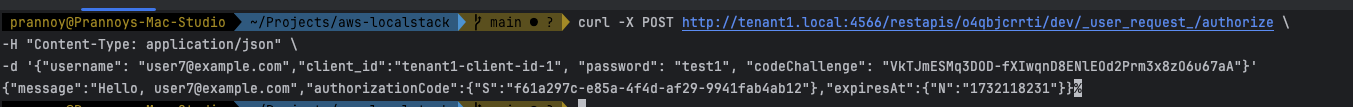
\includegraphics[width=\textwidth, height=60]{pics/authorize.png}} % Image with border
        \caption{Successful user Authorise for tenant1}
        \label{fig:authorize_tenant_1_success}
    \end{figure}

    \begin{figure}[!htbp]
        \centering
        {\setlength{\fboxrule}{2pt} % Border thickness
        \setlength{\fboxsep}{1pt}  % Space between image and border
        \fbox{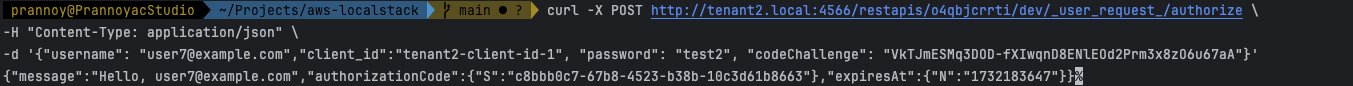
\includegraphics[width=\textwidth,height=55]{pics/authorize_tenant2_success.png}} % Image with border
        \caption{Successful user Authorise for tenant2)}
        \label{fig:authorize_tenant_2_success}
    \end{figure}

    \item \textbf{Authentication Failures:} Tested various failure scenarios to ensure the system handles them securely and as expected:
    \begin{itemize}
        \item \textbf{Invalid Credentials:} Attempted authentication with incorrect tenant credentials to confirm that the system denies access and provides appropriate error responses.
        
        \begin{figure}[!htbp]
            \centering
            {\setlength{\fboxrule}{2pt} % Border thickness
            \setlength{\fboxsep}{1pt}  % Space between image and border
            \fbox{ 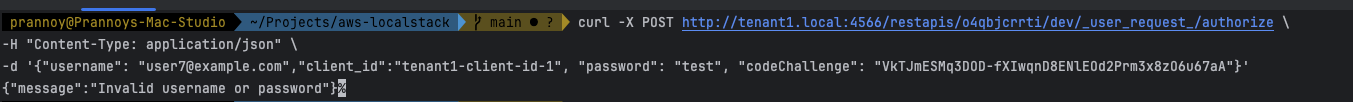
\includegraphics[width=\textwidth, height=60]{pics/authorize_wrong_pass.png}} % Image with border
            \caption{Unsuccessful user Authorise for tenant1 with wrong password}
            \label{fig:authorize_tenant_1_wrong_pass}
        \end{figure}

       
        \item \textbf{Unknown Client ID:} Tested requests with an unregistered or invalid client ID to confirm the endpoint rejects such requests without further processing.

        \begin{figure}[!htbp]
            \centering
            {\setlength{\fboxrule}{2pt} % Border thickness
             \setlength{\fboxsep}{1pt}  % Space between image and border
             \fbox{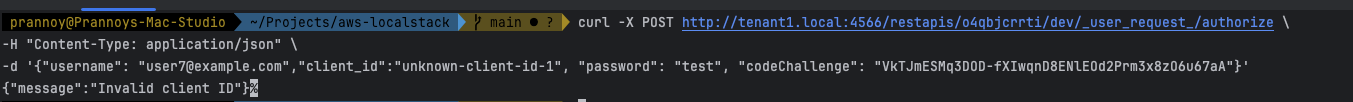
\includegraphics[width=\textwidth,height=60]{pics/authorize_unknown_client.png}} % Image with border
            \caption{Unsuccessful user Authorise for tenant1 with Unknown Client}
            \label{fig:authorize_tenant_1_unknown_client}
        \end{figure}
            
        \item \textbf{Missing Code Challenge:} Simulated a PKCE (Proof Key for Code Exchange) downgrade attack by omitting the \texttt{code\_challenge} parameter. This test was designed to ensure that the endpoint enforces PKCE requirements and denies the request if missing the \texttt{code\_challenge}.
        \begin{figure}[!htbp]
             \centering
             {\setlength{\fboxrule}{2pt} % Border thickness
             \setlength{\fboxsep}{1pt}  % Space between image and border
             \fbox{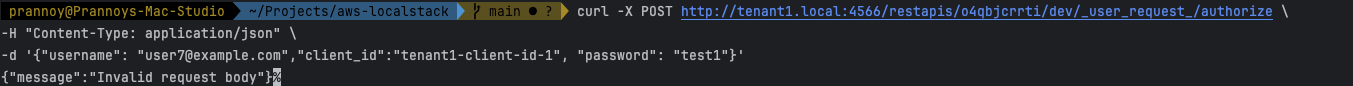
\includegraphics[width=\textwidth,height=55]{pics/authorize_without_code_challenge.png}} % Image with border
            \caption{Unsuccessful user Authorise for the tenant1 without Code Challenge (PKCE Downgrade)}
            \label{fig:authorize_tenant_1_without_code_challenge}
        \end{figure}

    \end{itemize}
\end{enumerate}

These tests helped validate the robustness of the \textbf{/authorize} endpoint, ensuring it functions correctly under normal conditions while effectively mitigating common security threats.


\subsubsection{Token Endpoint}
Manual tests were also conducted on the \textbf{/token} endpoint to verify its functionality and robustness. The following scenarios were tested:

\begin{enumerate}
    \item \textbf{Successful Token Retrieval:} Verified that the endpoint successfully issues tokens when provided with a valid authorisation code, client ID, and code verifier. The tokens are signed using an asymmetric key using the RS256 Algorithm (Refer to Figure \ref{fig:token_tenant_1_token_signed}). The private key is generated using the RSA-2048-bit algorithm (refer to Appendix \ref{apendix:create_private_keys}), and the keys are stored securely in the secrets manager, which the token lambda retrieves (Refer to Appendix \ref{apendix:token_signing}).

       \begin{figure}[!htbp]
             {\setlength{\fboxrule}{2pt} % Border thickness
             \setlength{\fboxsep}{1pt}  % Space between image and border
             \fbox{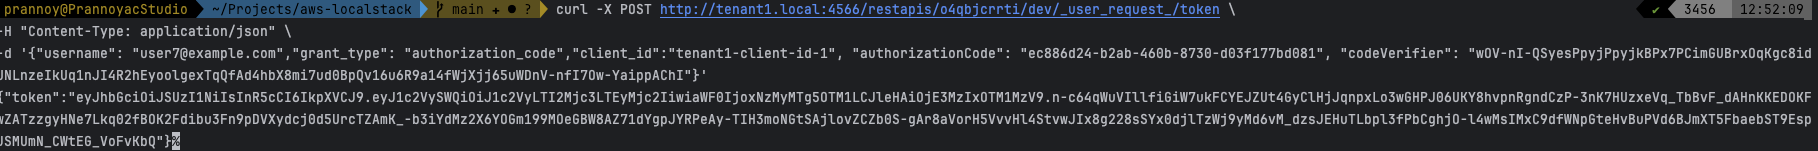
\includegraphics[width=\textwidth,height=50]{pics/token_successful_token.png}} % Image with border
            \caption{Successful token retrieval for tenant 1}
            \label{fig:token_tenant_1_success}
        \end{figure}

    \item \textbf{Expired Authorisation Code:} Attempted to retrieve a token using an expired authorisation code to ensure the endpoint denies the request with an appropriate error response.

\begin{figure}[!htbp]
             \centering
             {\setlength{\fboxrule}{2pt} % Border thickness
             \setlength{\fboxsep}{1pt}  % Space between image and border
             \fbox{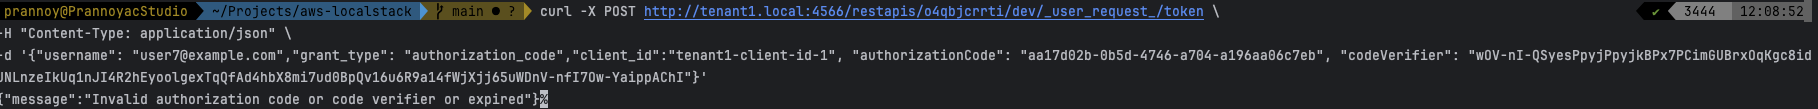
\includegraphics[width=\textwidth,height=50]{pics/token_auth_code_expired.png}} % Image with border
            \caption{Unsuccessful token retrieval as Authorisation Code expired}
            \label{fig:token_auth_code_expired}
        \end{figure}
        
    \item \textbf{Missing Code Verifier:} Simulated a scenario where the \texttt{code\_verifier} parameter was omitted during the token exchange. This test ensured that the endpoint rejects the request and enforces PKCE compliance.

    \begin{figure}[!htbp]
         \centering
         {\setlength{\fboxrule}{2pt} % Border thickness
         \setlength{\fboxsep}{1pt}  % Space between image and border
         \fbox{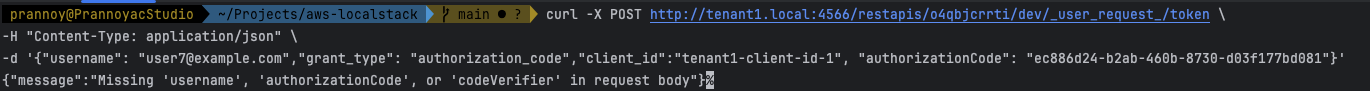
\includegraphics[width=\textwidth,height=50]{pics/token_without_code_veri.png}} % Image with border
        \caption{Unsuccessful token retrieval as no Code Verifier Present (PKCE Downgrade)}
        \label{fig:token_no_code_veri}
    \end{figure}

    \item \textbf{Missing \texttt{grant\_type}:} Sent a token exchange request without setting  \sloppy \seqsplit{grant\_type=authorization\_code}, confirming that the endpoint validates the presence of required parameters and returns a proper error if the \texttt{grant\_type} is missing or incorrect.

        \begin{figure}[!htbp]
         \centering
         {\setlength{\fboxrule}{2pt} % Border thickness
         \setlength{\fboxsep}{1pt}  % Space between image and border
         \fbox{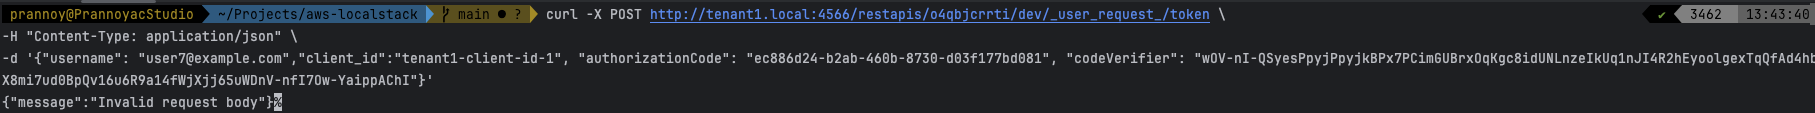
\includegraphics[width=\textwidth,height=50]{pics/token_missing_grant.png}} % Image with border
        \caption{Unsuccessful token retrieval as no Grant Type}
        \label{fig:token_no_grant_type}
    \end{figure}
\end{enumerate}

These tests validated the \textbf{/token} endpoint's ability to securely handle both successful and invalid requests, ensuring proper error handling for edge cases and enforcement of PKCE requirements.

\subsection{Automated Tests And Scans}
In addition to manual tests, various automated tests and security scans were conducted to ensure the application's robustness, security, and maintainability. The automated testing process included:

\begin{enumerate}
    \item \textbf{Unit Tests:} 
    Automated unit tests were implemented to validate the functionality of individual components of the \textbf{/authorize} and \textbf{/token} endpoints. These tests ensure that each component operates as intended, providing confidence in the correctness and reliability of the code. 

    The unit tests covered both the positive and negative scenarios for the business logic of the endpoints, verifying that:
    \begin{itemize}
        \item The \textbf{/authorize} endpoint correctly handles authentication requests, validates input parameters and securely generates authorisation codes.
        \item The \textbf{/token} endpoint properly exchanges authorisation codes for access tokens, enforces PKCE compliance and handles edge cases, such as expired or invalid codes.
    \end{itemize}
    
    As illustrated in Figure~\ref{fig:Unit Test}, the unit tests achieved a code coverage of approximately 97\%. This high level of coverage indicates that nearly all the application's critical paths and edge cases were thoroughly tested, ensuring functional correctness and robustness.

        \begin{figure}[!htbp]
         \centering
         {\setlength{\fboxrule}{2pt} % Border thickness
         \setlength{\fboxsep}{1pt}  % Space between image and border
         \fbox{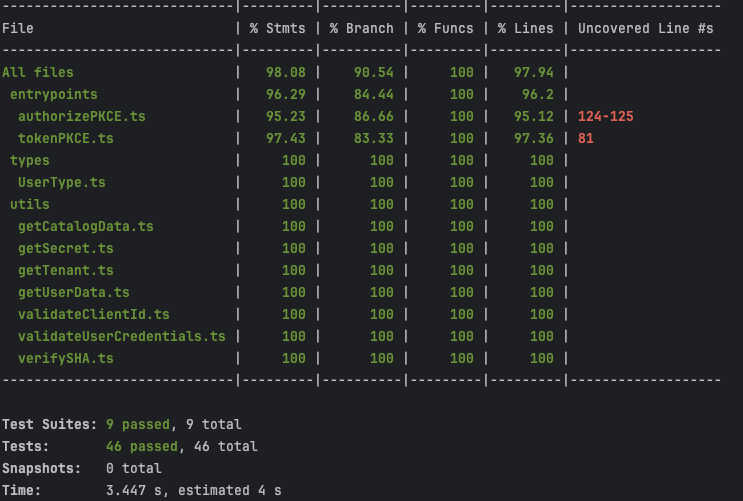
\includegraphics[width=\textwidth, height=200px]{pics/unit_test.png}} % Image with border
        \caption{Unit Test}
        \label{fig:Unit Test}
    \end{figure}

    \item \textbf{Fuzz Tests:} 
    Fuzz testing was conducted by sending random or malformed input to the \textbf{/token} endpoint to identify potential vulnerabilities, such as crashes, unexpected behaviour, or unhandled exceptions. This helps ensure the endpoint is resilient to invalid or malicious inputs.

    \item \textbf{Security Scans:}
    Security scans were employed to identify potential vulnerabilities and maintain best practices:
    \begin{itemize}
        \item \textbf{Code Linting with ESLint:} 
        ESLint was utlised to identify code smells and ensure the codebase adhered to clean coding principles and established security best practices. Linting is crucial in minimizing the risk of introducing vulnerabilities by enforcing consistent code quality. The eslint-plugin-security-node plugin was used to enhance this process, which proved to be highly effective in detecting common security issues and code smells. Its integration ensured a more robust and secure codebase by proactively addressing potential weaknesses. Figure \ref{fig:lint_results} depicts the results of some code smells detected using the linter. 

                \begin{figure}[!htbp]
                     \centering
                     {\setlength{\fboxrule}{2pt} % Border thickness
                     \setlength{\fboxsep}{1pt}  % Space between image and border
                     \fbox{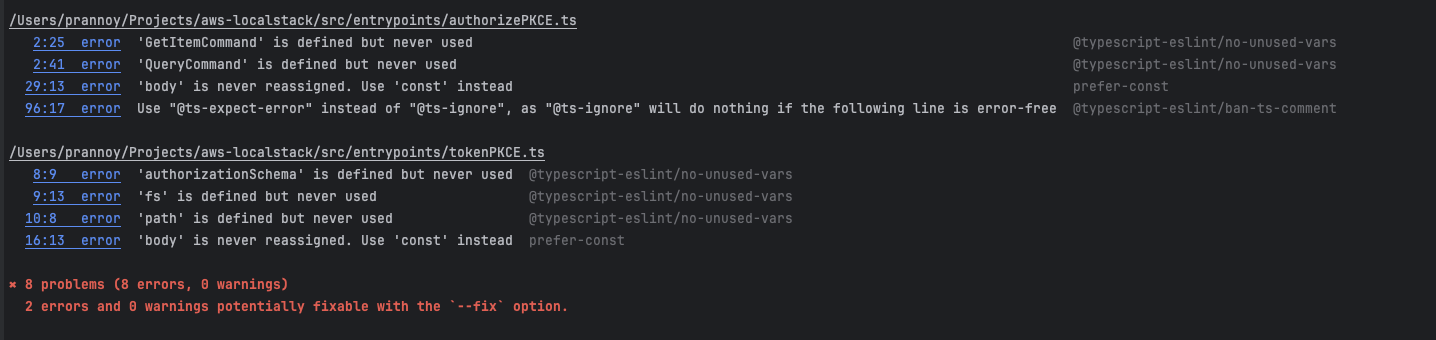
\includegraphics[width=\textwidth, height=200px]{pics/linting.png}} % Image with border
                    \caption{Lint results}
                    \label{fig:lint_results}
                \end{figure}


        \item \textbf{Cloud Infrastructure Scanning with Prowler:} 
        Prowler is a versatile open-source tool designed to scan cloud providers like AWS, helping identify potential misconfigurations in cloud infrastructure. It provides critical insights into security risks, such as overly permissive IAM roles, improper or missing logging configurations, and inadequate encryption settings. One of the critical strengths of Prowler is its ability to not only detect these issues but also provide actionable recommendations and remedies to address the identified misconfigurations. For example, as shown in Figure \ref{fig:prowler_results}, the tool detected 14 medium-level misconfigurations, each accompanied by specific remediation steps to mitigate the associated risks.

                \begin{figure}[!htbp]
                     \centering
                     {\setlength{\fboxrule}{2pt} % Border thickness
                     \setlength{\fboxsep}{1pt}  % Space between image and border
                     \fbox{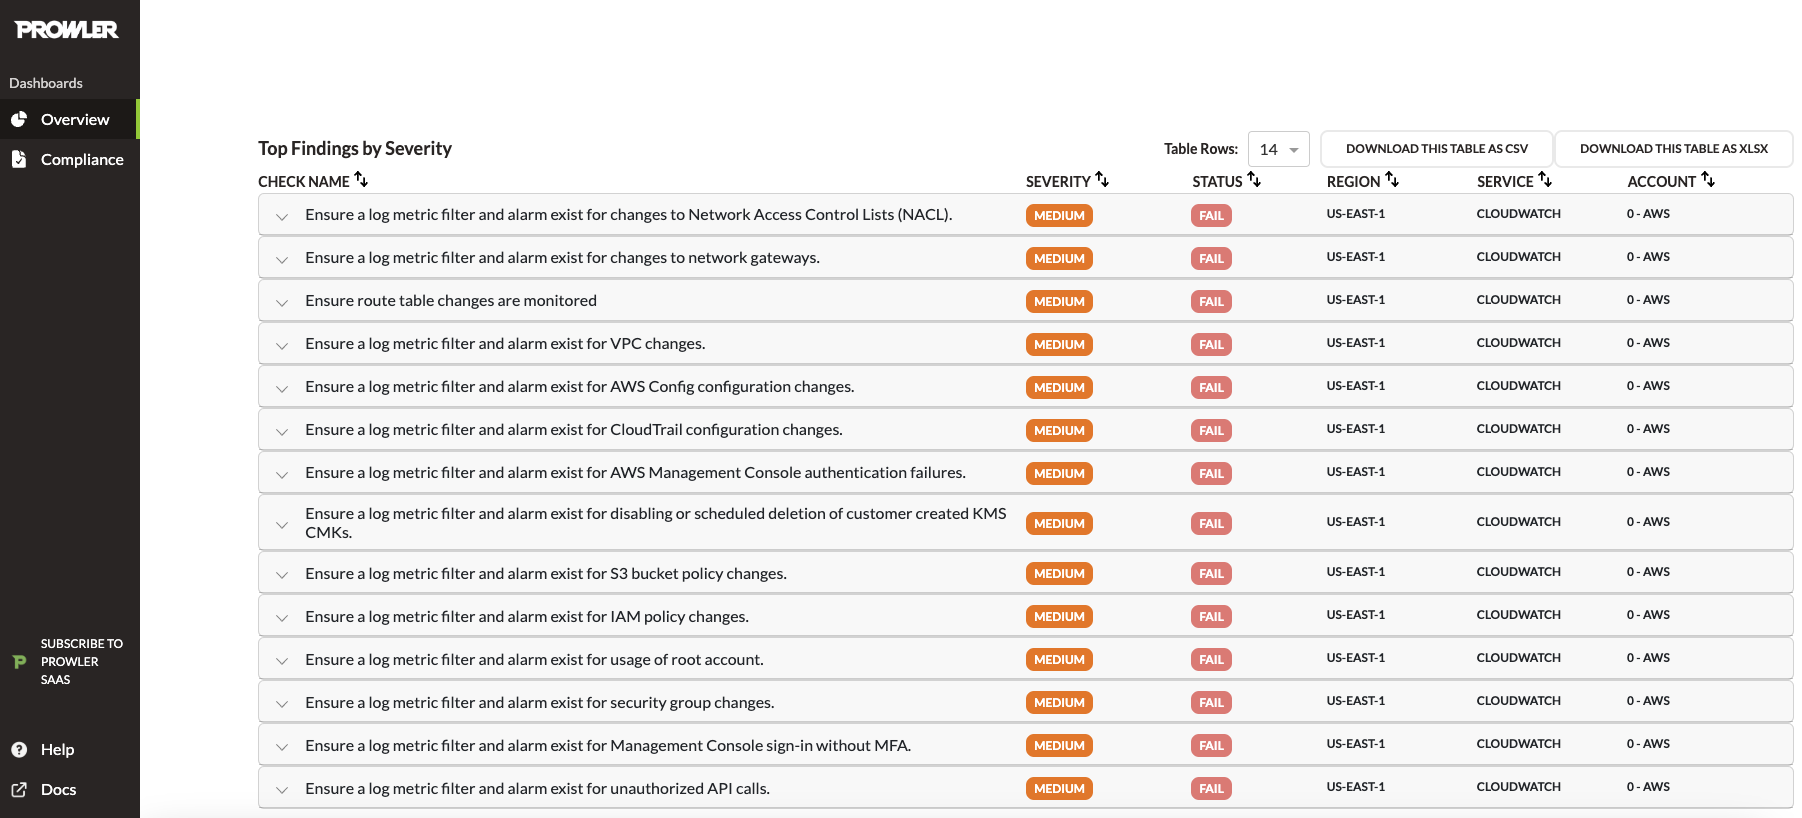
\includegraphics[width=\textwidth, height=120px]{pics/prowler.png}} % Image with border
                    \caption{Prowler Scan result}
                    \label{fig:prowler_results}
                \end{figure}

        \newpage
        In addition to the standard security checks, Prowler extends its functionality to compliance auditing. It supports testing against various industry standards, offering organisations a way to assess and strengthen their compliance posture. In this context, Prowler was utlised to perform both cloud infrastructure scans and compliance checks for ISO 27001:2013 (refer to Figure \ref{fig:prowler_iso_results}) and GDPR (refer to Figure \ref{fig:prowler_gdpr_results}). These compliance scans are particularly valuable for organisations that adhere to regulatory requirements or maintain certifications, as they provide a comprehensive view of potential gaps and actionable insights for achieving compliance.
        
                \begin{figure}[!htbp]
                     \centering
                     {\setlength{\fboxrule}{2pt} % Border thickness
                     \setlength{\fboxsep}{1pt}  % Space between image and border
                     \fbox{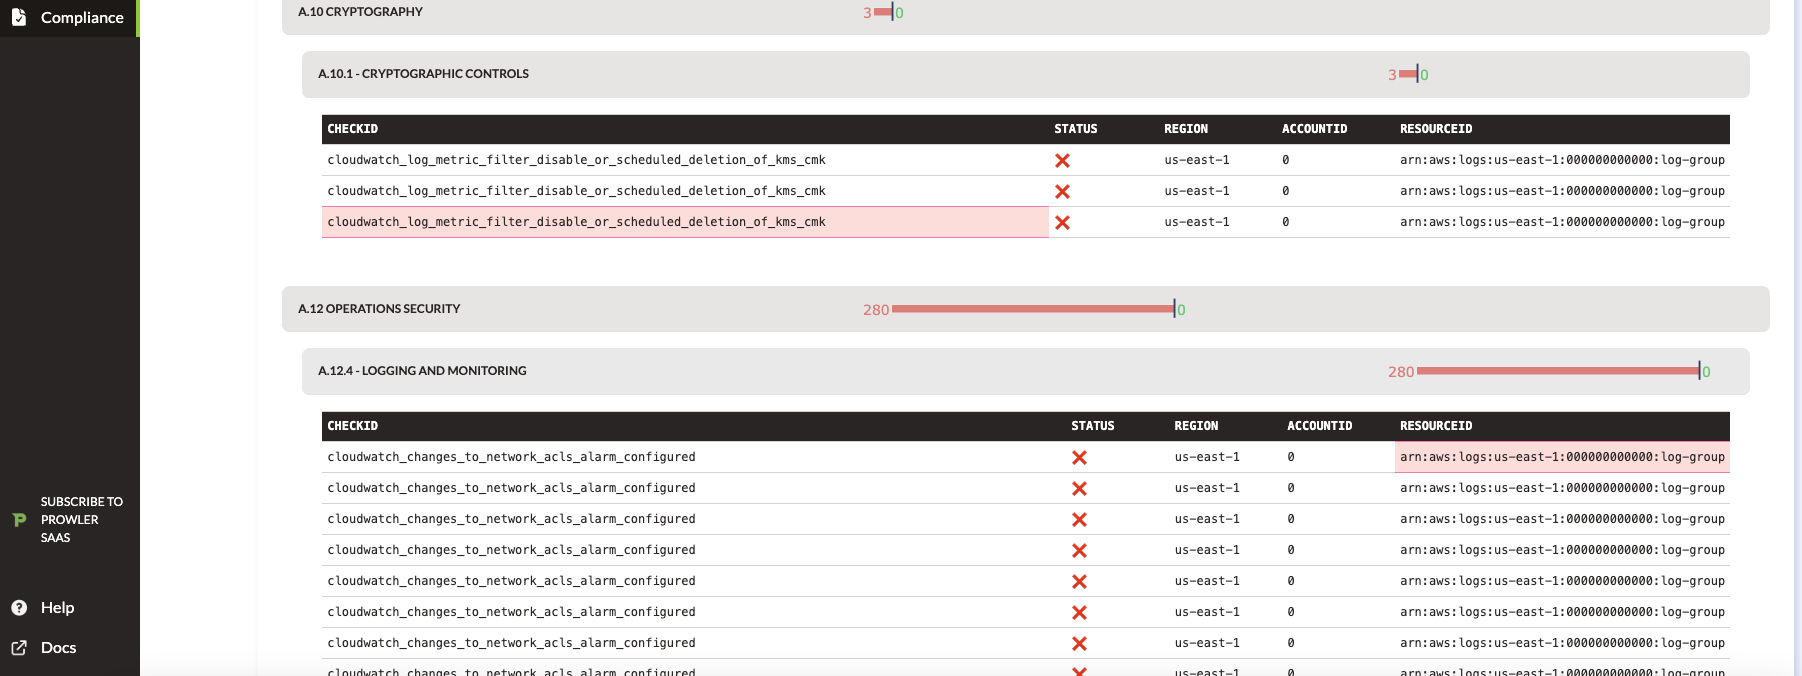
\includegraphics[width=\textwidth, height=150px]{pics/prowler_iso.png}} % Image with border
                    \caption{Prowler ISO:27001:2013 Scan result}
                    \label{fig:prowler_iso_results}
                \end{figure}

                \begin{figure}[!htbp]
                     \centering
                     {\setlength{\fboxrule}{2pt} % Border thickness
                     \setlength{\fboxsep}{1pt}  % Space between image and border
                     \fbox{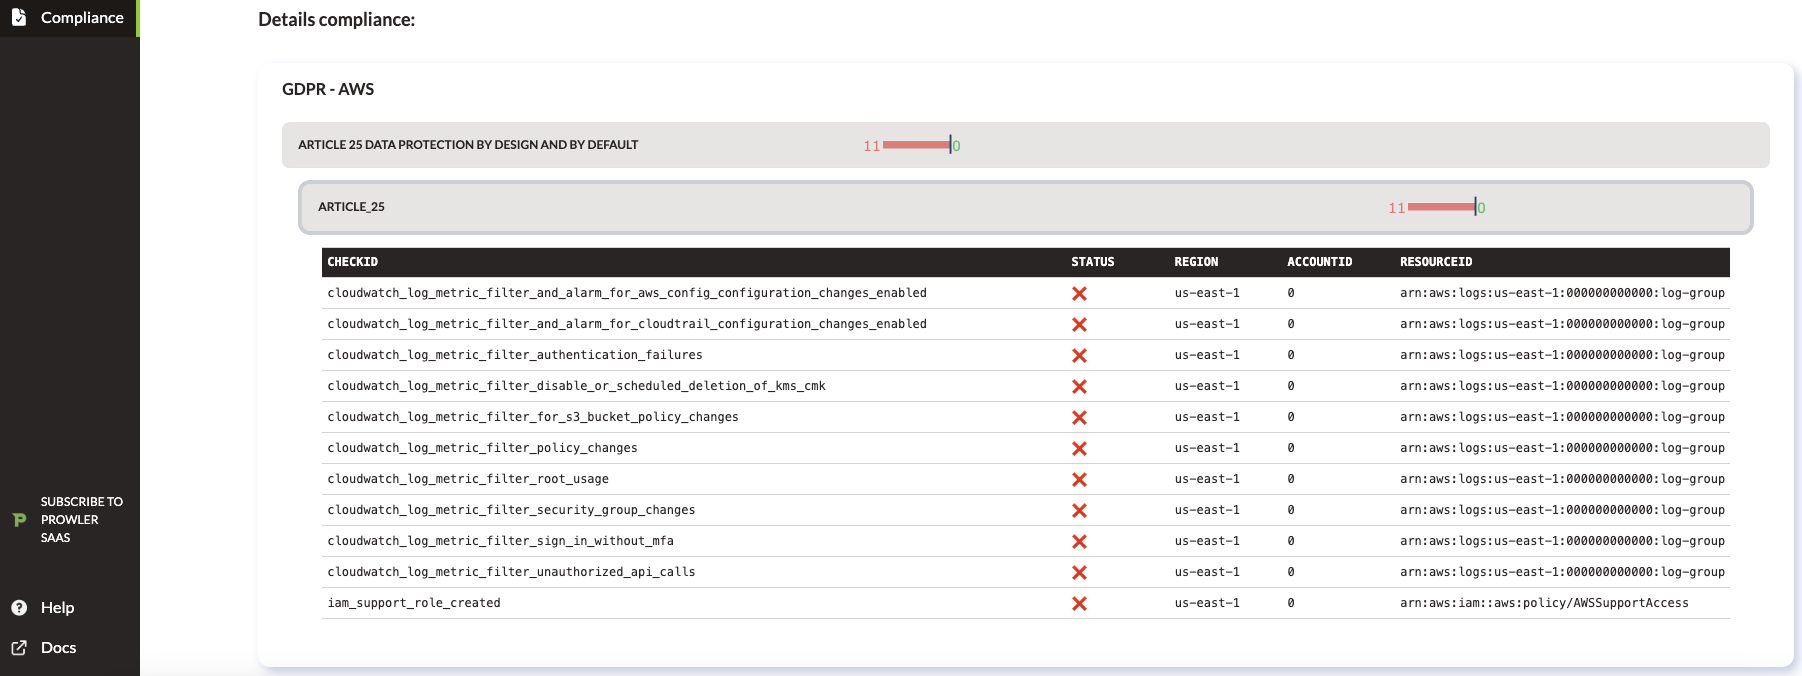
\includegraphics[width=\textwidth, height=150px]{pics/prowler_gpdr.png}} % Image with border
                    \caption{Prowler GDPR Scan result}
                    \label{fig:prowler_gdpr_results}
                \end{figure}
        By integrating security scanning with compliance testing, Prowler is a powerful tool for proactively securing cloud environments and aligning with best practices.        
    \end{itemize}
    \item \textbf{Static Code Analysis with Snyk:} Snyk is utlised in this project as a static analysis tool to detect vulnerabilities, improve code quality, and ensure secure development practices. It complements \texttt{ESLint} by focusing on security flaws in business logic and Infrastructure-as-Code (IaC). While \texttt{ESLint} enforces coding standards and detects bugs in JavaScript, Snyk extends the scope by scanning for vulnerabilities in dependencies, IaC configurations, and container images. This integration ensures both high-quality code and robust security measures. Figure \ref{fig:snyk_results} illustrates the results of Snyk's analysis.
    

    \begin{figure}[!htbp]
                     \centering
                     {\setlength{\fboxrule}{2pt} % Border thickness
                     \setlength{\fboxsep}{1pt}  % Space between image and border
                     \fbox{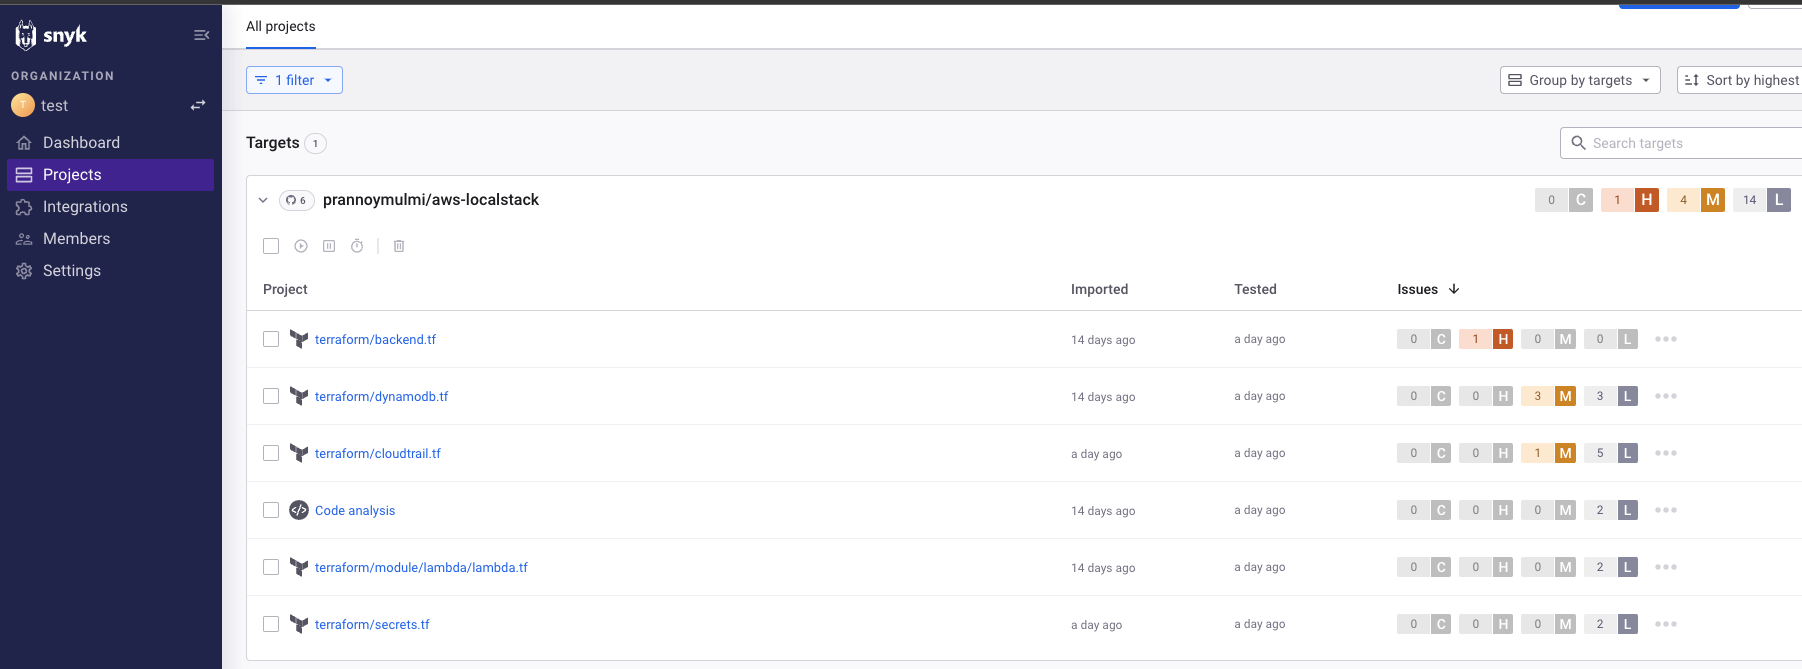
\includegraphics[width=\textwidth]{pics/snyk.png}} % Image with border
                    \caption{Static Code Analysis with Snyk}
                    \label{fig:snyk_results}
                \end{figure}
\end{enumerate}

\section{Results} 

\subsection{Cloud Configuration: A Top Security Concern}

In this analysis, the misconfiguration of cloud services emerged as one of the most significant issues. This finding was supported by vulnerability scans conducted using \textbf{Prowler} and \textbf{Snyk}, which identified multiple configuration-related warnings and vulnerabilities across the actively used cloud services: \textbf{Amazon DynamoDB}, \textbf{Amazon API Gateway (APIGW)}, and \textbf{AWS Lambda}.

\paragraph{Security Scan Results}
\begin{itemize}
    \item \textbf{Prowler}: Prowler flagged \textbf{14 medium-severity warnings} and \textbf{1 high-severity warning} within the scanned cloud configurations. These issues highlight potential risks that could expose the environment to unauthorised access or reduce its resilience to attacks.
    \item \textbf{Snyk}: Snyk detected \textbf{1 high-severity issue}, \textbf{4 medium-severity vulnerabilities}, and \textbf{1 low-severity issue}. These findings further corroborate the need for a robust approach to managing cloud configuration risks.
\end{itemize}

\paragraph{Complexity and Scaling Risks}
The scans were conducted for only three actively used AWS services: \textbf{DynamoDB}, \textbf{APIGW}, and \textbf{Lambda}, which represent a subset of a typical cloud environment. Despite the limited scope, the results already highlight significant concerns about misconfiguration. As the number of services grows and their interdependencies increase, the complexity of managing cloud configurations will scale significantly. This growth will likely lead to an even greater risk of misconfigurations, amplifying the potential attack surface.

Following the finding, it is necessary to emphasize that \textbf{cloud configurations represent a critical security threat}. This aligns with the assessment outlined in \ref{table:threat_model_assets}, where misconfiguration was identified as one of the top-ranked threats to the cloud environment. Misconfigured resources can lead to data breaches, service disruptions, and compliance violations, underscoring the importance of proactive configuration management and continuous monitoring.


\subsection{Security Tools: Useful but Not Sufficient}

Security tools such as \textbf{Prowler} and \textbf{Snyk} provide valuable insights into potential vulnerabilities and misconfigurations within cloud environments. However, while these tools are effective for identifying numerous issues, they cannot be solely relied upon for ensuring a secure setup. Several limitations and shortcomings were observed during the analysis, highlighting the importance of complementing automated tools with reviews from an expert and adherence to security best practices.

\paragraph{Undetected Security Issues}

Despite their advantages, the tools failed to detect certain critical issues deliberately introduced into the environment for testing purposes. These include:

\begin{itemize}
    \item \textbf{IAM Policy Not Following the Principle of Least Privilege}: 
    A deliberately misconfigured IAM policy that violated the principle of least privilege (refer to Listing \ref{lst:bad_policy_iam}) was created as part of the test. Such a policy, if accessed by a malicious actor, could be exploited to gain elevated privileges and compromise the environment. However, this misconfiguration or bad practice was not flagged by any of the tools used in this study.

    \begin{lstlisting}[caption={Added a Bad IAM Policy that allows all actions}, label={lst:bad_policy_iam}]
# IAM Policy for Lambda to log to CloudWatch
resource "aws_iam_policy" "test_bad_policy" {
  name        = "bad policy"
  description = "IAM policy test for bad example"

  policy = jsonencode({
    Version = "2012-10-17",
    Statement = [
      {
        Effect = "Allow",
        Action = [
          "*:*"
        ],
        Resource = "*"
      }
    ]
  })
}
\end{lstlisting} 

\item \textbf{False Positives and Contextual Irrelevance}: Besides undetected issues, the tools occasionally generated \textbf{false positives} or flagged findings irrelevant to the specific use case. For instance, Prowler flagged the absence of a \texttt{support\_role} as a medium-severity issue. However, no support role was required for the use case tested, and this finding was irrelevant. Such false positives can create unnecessary noise in the results. An increase of noise in such tools could train teams to treat warnings from the tools as noise, and this could lead to an overlook of critical issues.
\end{itemize}

\subsection{Threats in OIDC and Cloud Integration}
Several well-documented threats, such as token-related risks, replay attacks, and phishing, remain critical to access in OIDC as they pose significant risks if not taken care of. Furthermore, these threats become even more significant when integrated with cloud environments, where additional complexities arise.

The complexities increase as many cloud providers offer vast services like databases, networking solutions, and application hosting. This flexibility increases the chance of choosing the wrong service and requires good knowledge of the different services. A poorly informed choice of infrastructure or security settings can inadvertently expose sensitive data, including Personally Identifiable Information (PII), to unauthorised access.

These scenarios can have severe consequences, including data leaks and regulatory violations. For example, mismanagement of access controls or insecure handling of tokens in cloud services could lead to unauthorised access. Such vulnerabilities compromise data protection and violate the regulatory framework. Namely, GDPR Article 25 and GDPR Article 32 (Refer to Section \ref{section:gdpr}) mandate "data protection by design and by default," emphasizing the importance of embedding robust safeguards into systems from the outset and proper security measures that should be taken to protect sensitive data. The risks associated with OIDC-specific and cloud-specific vulnerabilities highlight the need for heightened oversight to prevent breaches and ensure compliance with legal and regulatory standards.


      